%
%
% Relatório 2 - Seguranca de Redes
% João Fiuza de Alencastro - 15/0131933
%
%

\documentclass[journal]{IEEEtran}
\usepackage[utf8]{inputenc}
\usepackage{graphicx}
\usepackage{hyperref}

\begin{document}
%
% paper title
\title{Ataques (básicos) a uma rede local}

\author{João~Fiuza~de~Alencastro~15/0131933}%

\maketitle

\begin{abstract}
Este relatório não tem um ataque principal em questão, aqui é onde comecamos a falar sobre ataques simples em geral, ataques conhecidos, como, por exemplo, \textit{Gathering, DoS, Flood,} entre outros.
\end{abstract}

% Note that keywords are not normally used for peerreview papers.
\begin{IEEEkeywords}
Ataques, redes, LAN, ARP, DDoS, Gathering, Flood, BruteForce, HTTP, IP, NMap, Python3.
\end{IEEEkeywords}




\section{Introduction}

\IEEEPARstart{O}{s} ataques mencionados a cima são somente o primeiro passo para ataques maiores. Por esse motivo, ataques simples podem acabar se tornando extremamente perigosos. \par
Uma das principais solucões para ataques externos é a implementação de uma IDS (Invasion Detection System), uma aplicação, normalmente local, que monitora a rede ou os sistemas à procura de invasores ou softwares maliciosos. \par
Abaixo são apresentados alguns dos principais ataques que já foram muito bem sucedidos no passado e continuam sendo efetivos em sistemas mais vulneráveis.



\subsection{NMap}
Tema já abordado no relatório NMap[1], porém de extrema importância para o processo de \textit{'information Gathering'}. Também conhecido como Port Scanner, o NMap pode almejar de sistemas a redes inteiras e é já é utilizado por diversos frameworks conhecidos.

\subsection{Flood}
A proposta do \textit{Flood}, como o nome já indica, é encher/"entupir" algo ou alguém com algo. Imaginemos uma analogia básica para fins didáticos, um atendente de bar, por exemplo, está trabalhando em uma noite especial e 100 pessoas tentam fazer pedidos simultaneamente para ele, sem dúvida alguma, ele não conseguirá lidar com toda essa demanda e talvez até desista da tarefa. Pois, esse é o princípio do \textit{Flood}, enviar pedidos em larga escala em um curto período de tempo.

\subsection{DoS (Denial of Service)}
%DoS
O ataque de negação de serviço utiliza-se do princípio do \textit{Flood}, entupindo os recursos de um serviço com requisições, indisponibilizando aos usuários daquele serviço acesso e comunicação. \par
No experimento realizado, um simples script em python foi o suficiente para simular um pequeno ataque DoS ao serviço criado pelo colega próximo do laboratório, conectado à mesma LAN. O serviço era uma pequena aplicação HTTP na porta 8000 e o script cria 300 conexões HTTP.\par
Na imagem abaixo, pode ser visto que o IP da máquina localhost é 172.16.5.93 e foi feito um ataque DoS no endereço IP 172.16.5.91. Pode-se confirmar que o ataque foi bem sucedido, pois a resposta HTTP é um código 200, indicando sucesso. O número na linha logo abaixo do código 200 há um número que se repete, 715, este número representa o número de bytes no diretório no qual a aplicação está diretamente associado. 

%Imagem
\begin{figure}[h!]
	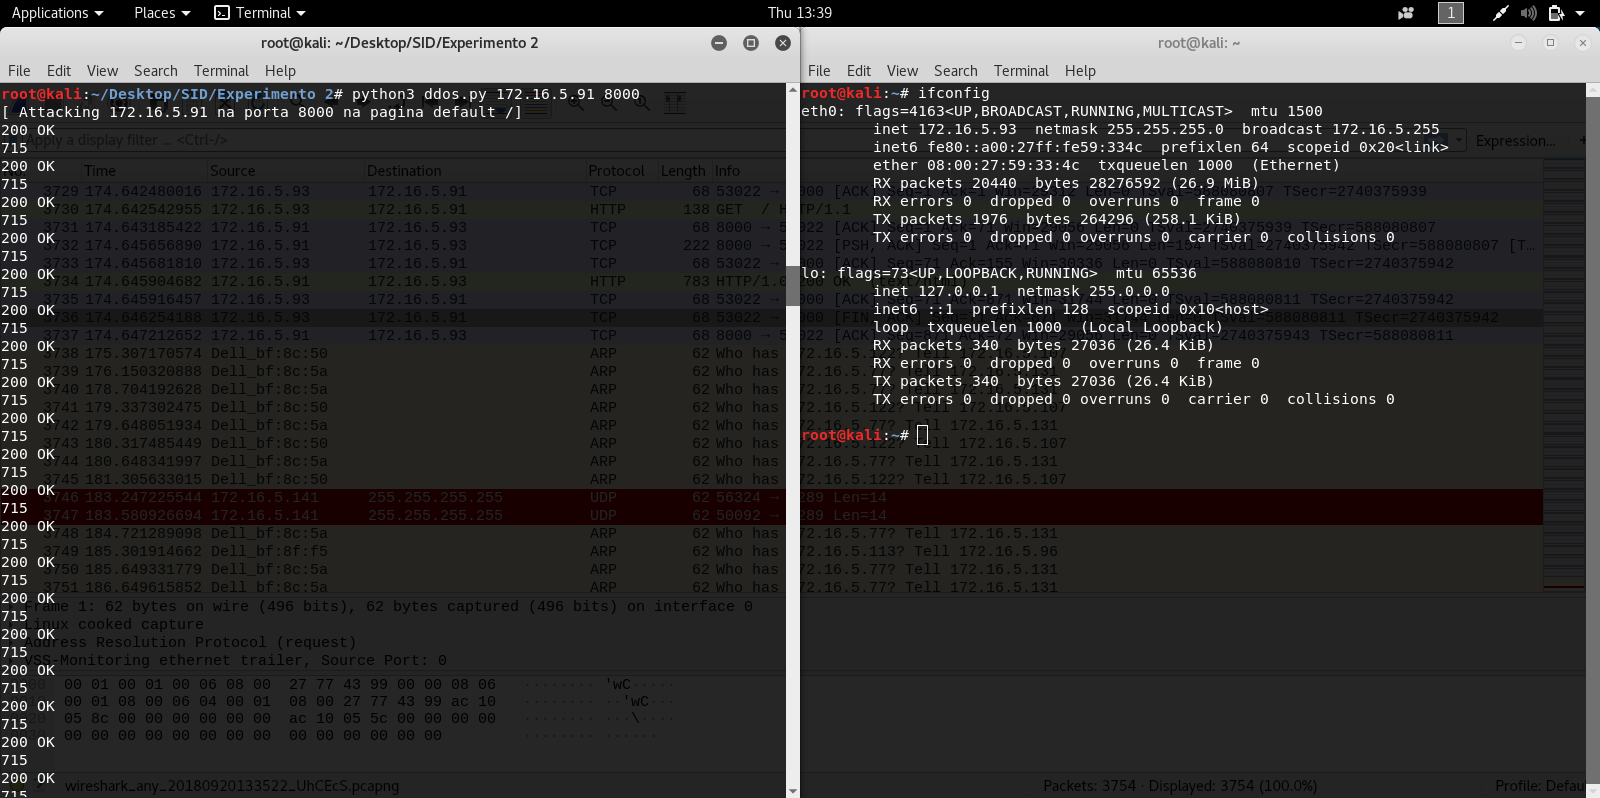
\includegraphics[width=\linewidth]{../fotos_experimento_2/atacandoRodrigo.png}
	\caption{Ataque DoS ao colega em mesma LAN}
	\label{fig:Ataque_a_terceiro}
\end{figure}

Na figura seguinte, podemos ver um mesmo ataque acontecendo, porém agora no próprio localhost, ou seja, em um serviço criado na mesma máquina atacante. Nessa imagem, é possível ver as requisições do lado do servidor, onde há informações do endereço IP do cliente, timestamp da requisição e o tipo da requisição, nesse caso o log do serviço é esse, porém pode ser muito diferente dependendo da aplicação. Perceba também, que o intervalo entre uma requisição e outra é tão pequena que todas na tela do terminal apresentam mesmo timestamp.

%Imagem
\begin{figure}[h!]
	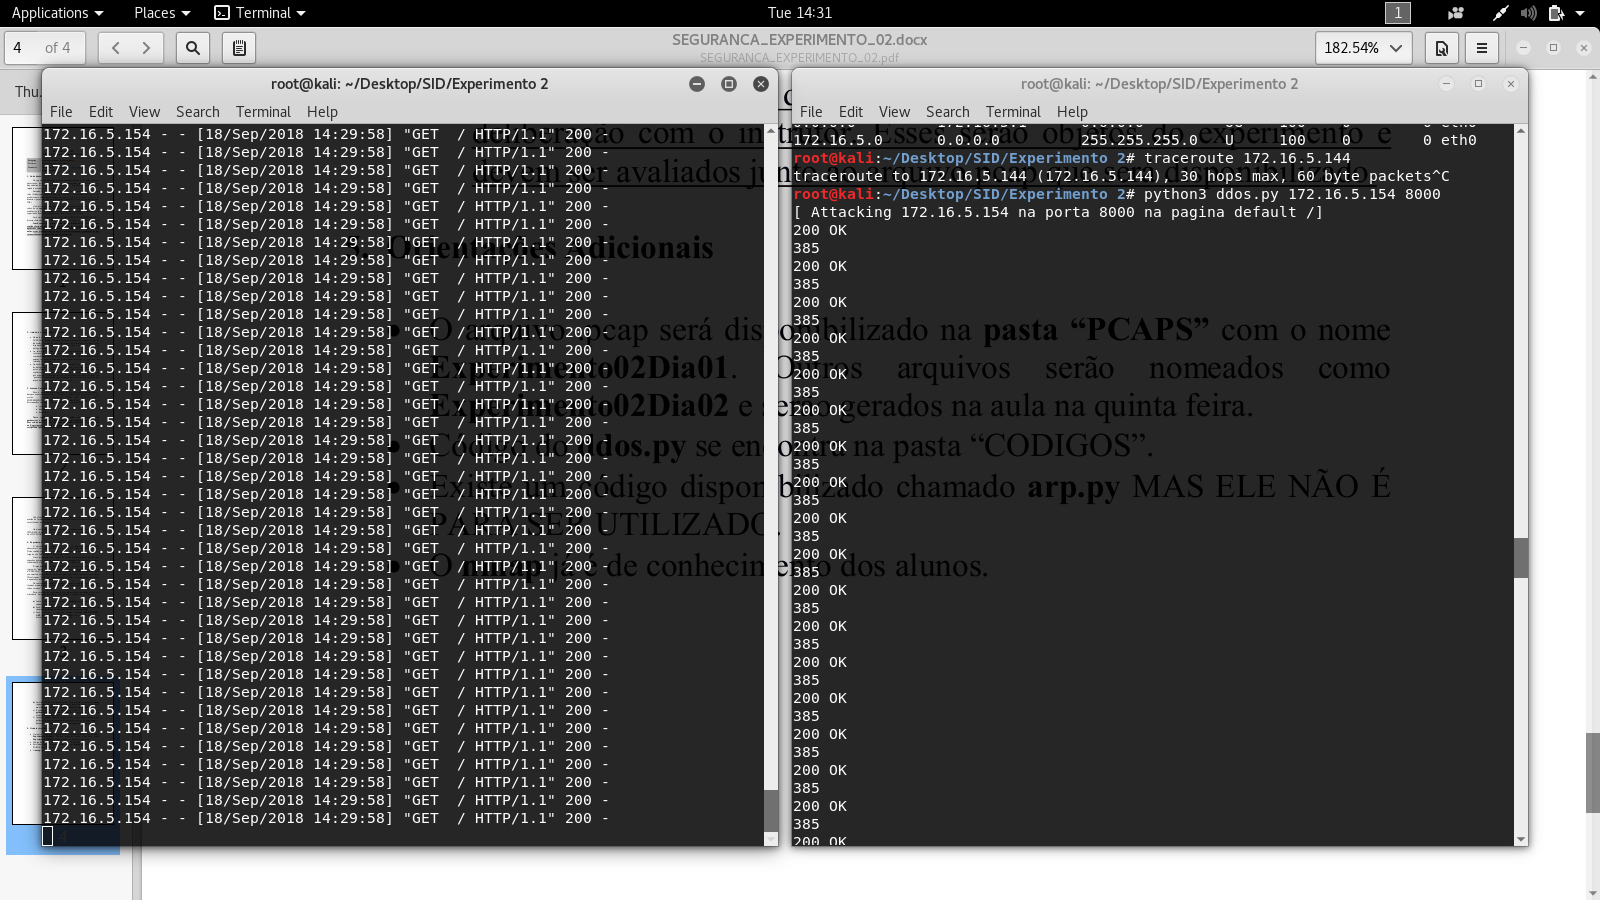
\includegraphics[width=\linewidth]{../fotos_experimento_2/atacandoLocalhost.png}
	\caption{Ataque DoS ao próprio endereço local}
	\label{fig:Ataque_a_si}
\end{figure}

Ao analisar o tráfego da rede, fica claro como um ataque de negação de serviço acaba sendo muito custoso para conexões TCP, já que para requisição HTTP, até mesmo um simples 'GET', requer um 'three-way-handshake' da conexão segura fornecida pelo TCP. Na figura abaixo podemos ver um pequeno pedaço da análise do tráfego em modo promíscuo no WireShark no exato momento do ataque.

%Imagem
\begin{figure}[h!]
	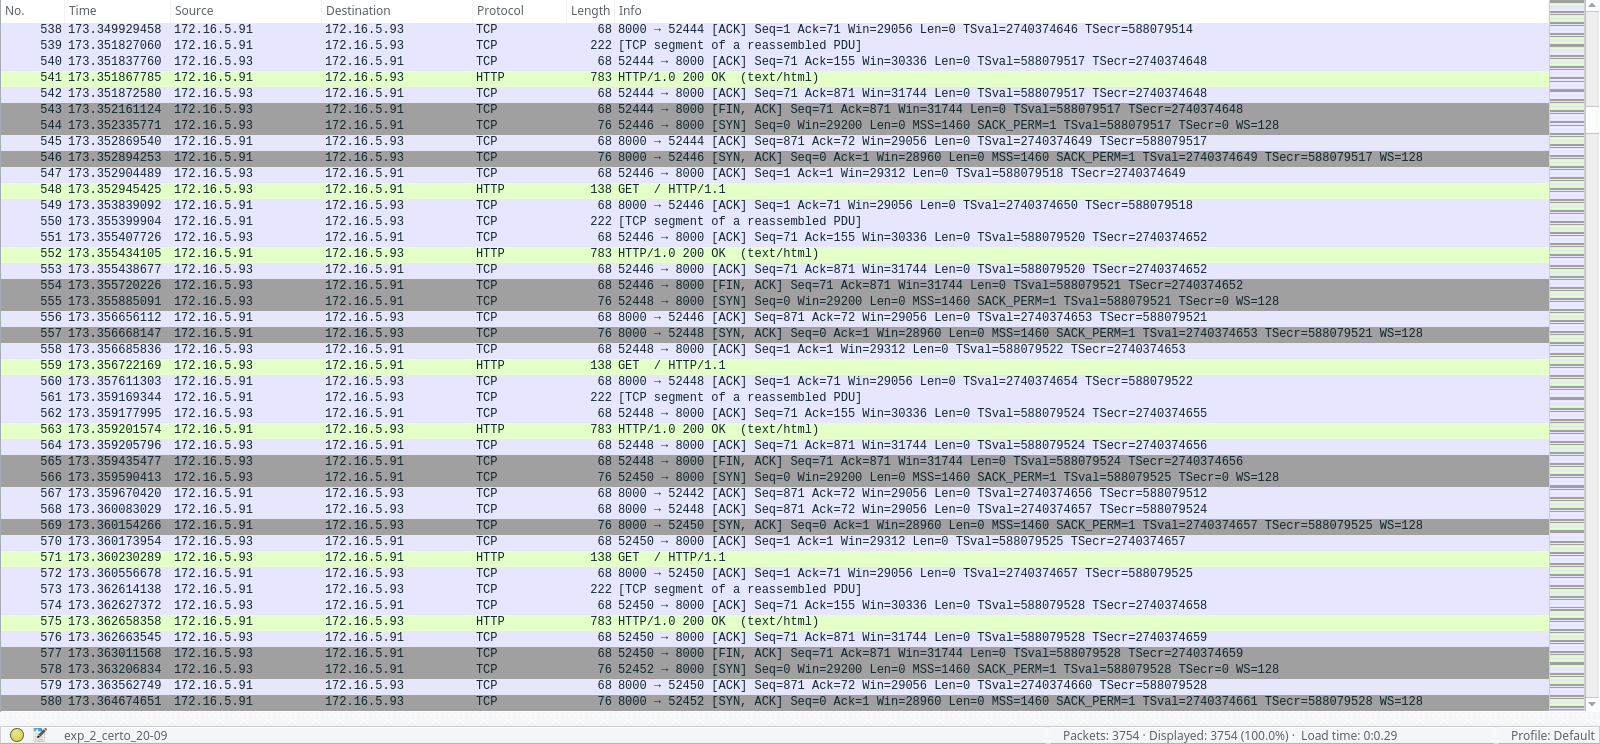
\includegraphics[width=\linewidth]{../fotos_experimento_2/pacotes_DoS_TCP_HTTP.png}
	\caption{Pacotes ataque DoS}
	\label{fig:Pacotes_ataque}
\end{figure}

%DDoS
O DDoS continua sendo um ataque de negação de serviço da mesma forma, porém mais "inteligente", já que ele distribui a origem do ataque, fazendo com que várias máquinas diferentes façam algumas poucas requisições, totalizando em um ataque generalizado e bem organizado. A maior vantagem do ataque ser distribuído dessa forma, é que o atacante gera uma dificuldade de localização grande, já que as requisições não são de um único endereço IP. Além disso, um ataque com várias máquinas dispõem de muito mais recursos do que somente uma máquina gerando requisições.

%Imagem
\begin{figure}[h!]
	\includegraphics[width=\linewidth]{../fotos_experimento_2/DDos_Attack.png}
	\caption{Topologia clássica de um DDoS distribuído}
	\label{fig:ddos}
\end{figure}

% An example of a floating figure using the graphicx package.
% Note that \label must occur AFTER (or within) \caption.
% For figures, \caption should occur after the \includegraphics.
% Note that IEEEtran v1.7 and later has special internal code that
% is designed to preserve the operation of \label within \caption
% even when the captionsoff option is in effect. However, because
% of issues like this, it may be the safest practice to put all your
% \label just after \caption rather than within \caption{}.
%
% Reminder: the "draftcls" or "draftclsnofoot", not "draft", class
% option should be used if it is desired that the figures are to be
% displayed while in draft mode.
%
%\begin{figure}[!t]
%\centering
%\includegraphics[width=2.5in]{myfigure}
% where an .eps filename suffix will be assumed under latex, 
% and a .pdf suffix will be assumed for pdflatex; or what has been declared
% via \DeclareGraphicsExtensions.
%\caption{Simulation Results.}
%\label{fig_sim}
%\end{figure}

% Note that IEEE typically puts floats only at the top, even when this
% results in a large percentage of a column being occupied by floats.


% Note that IEEE does not put floats in the very first column - or typically
% anywhere on the first page for that matter. Also, in-text middle ("here")
% positioning is not used. Most IEEE journals use top floats exclusively.
% Note that, LaTeX2e, unlike IEEE journals, places footnotes above bottom
% floats. This can be corrected via the \fnbelowfloat command of the
% stfloats package.



\section{Conclusion}
%DoS não distribuídos são extremamente ineficazes, pois hoje a grande maioria das aplicações podem detectar grandes volumes de requisições originadas em um mesmo IP ou poucos mesmos IPs.


% Ataque custoso para o atacate também
Excluindo as descobertas de vulnerabilidades, ataques de \textit{Flood} são, usualmente, custosos para o atacante também. Eles comprometem as conexões de um certo serviço, porém seus recursos ficam inutilizáveis. Por este motivo, hoje, atacantes utilizam-se de máquina alheias espalhadas pelo globo para realizar ataques distribuídos. E esse processo acontece, na maioria das vezes, sem o consentimento do dono da máquina, às vezes por ele baixar uma aplicação de fontes não confiáveis. \par

%IDS
Ataques de negação de serviço podem ser prevenidos por utilização de IDS (Invasion Detection System) em sua rede ou sistema. É necessário que haja algum processo específico para a detecção de intrusos ou atividades suspeitas, o caso do DoS. Ele pode ser o responsável por "perceber" múltiplas requisições, enviadas em um tempo realizável somente por máquinas, e deve ser capaz de "negar" o serviço demandado, e assim surge o nome do ataque.

%ATUALIZACOES DOS SOFTWARES



\begin{thebibliography}{1}

\bibitem{IDS}
https://en.wikipedia.org/wiki/Intrusion-detection-system
\bibitem{negacao_de_servico}
https://pt.wikipedia.org/wiki/Ataque-de-negacao-de-servico

\end{thebibliography}


\end{document}


